% Subsystem Report for the Analog Input Module system.
\fancyfoot[R]{WT}
\section[Analog Input]{Analog Input Module Subsystem}
\subsection{Description}
The purpose of the signal conditioning subsystem is to scale the analogue input
 to an appropriate level so that it can be read by the analogue to digital 
converter. The goal is to scale the output voltage to be between 0 and 5 volts 
and allow proper shifting and amplification via user interaction with the 
software.

 \begin{figure}[hbp]
\caption{Photograph of implemented signal conditioner on breadboard}
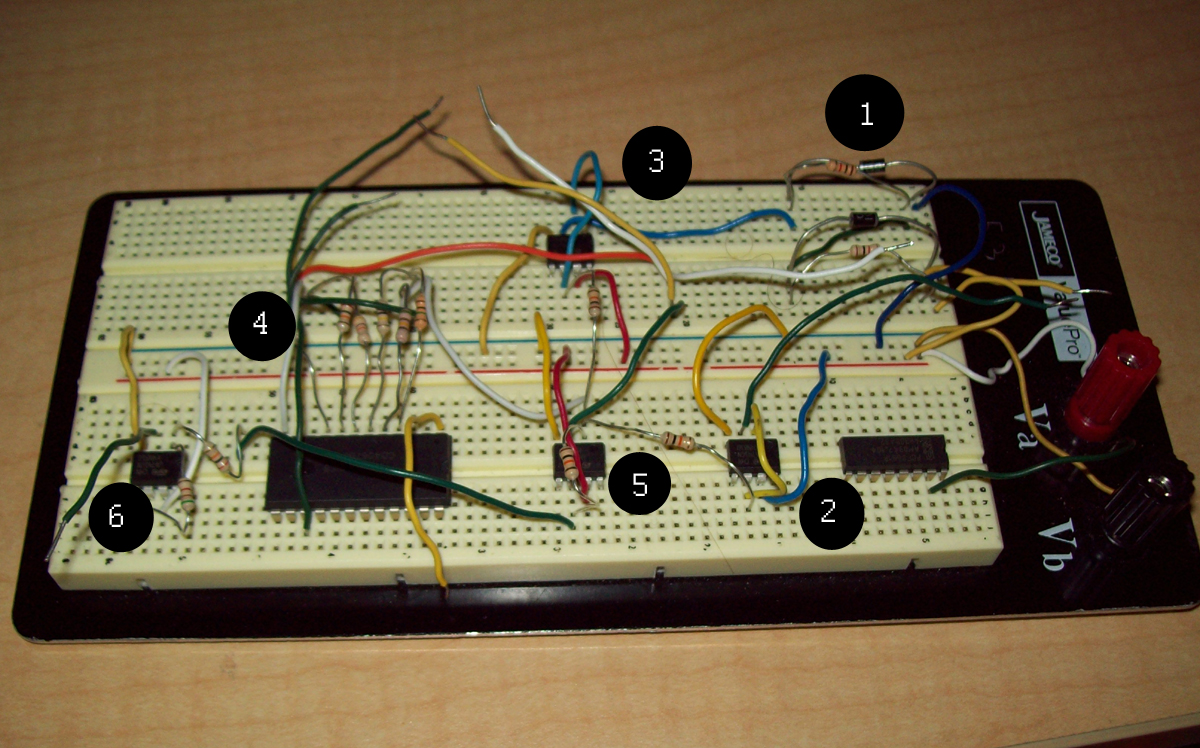
\includegraphics[width=5in]{sub_analog_hw.jpg}
\label{fig:analog breadboard}
\end{figure}


As per Figure \ref{fig:analog drawing}, this was implemented using 4 
operational amplifiers, a digital to analogue converter, a multiplexer, 
resistors, and diodes. 741 operational amplifiers were chosen for this circuit 
because they are the most inexpensive op amps to purchase and their specs allow
 for them to be used in this circuit. A reference voltage of +/- 12 volts was 
used to supply these op amps, which allow for a maximum of +/- 22 
volts\cite{ds:741-op-amp}.

The input voltage is allowed to range from -12.7 volts to +12.7 volts. The 
diode and resistor configuration shown in drawing 201 assures the input voltage
 cannot vary outside of this range. These standard diodes and resistors were 
chosen because only basic diodes and resistors were needed and these components
 were very inexpensive. This input voltage is applied to the non-inverting 
input of an operational amplifier. The output of this op amp goes back to the 
inverting op amp, so it acts as a voltage follower\cite{bk:olia}.

Another voltage is produced from a digital to analogue converter. This voltage
 ranges from 0 to 5 volts. The purpose of the digital to analogue converter is
 to shift the signal up and down. The user controls this shift using the
 software on the computer. Because this requires communication with the micro
 controller, a digital to analogue converter was chosen with an 
I$^2$C interface. Consequently the PCF8591 was selected to 
produce a voltage ranging from 0 to 5 that goes into the non-inverting input 
of an op amp. This op amp also acts as a voltage follower.

These 2 voltages were each placed in series with a 10k resistor and both 
connected to the inverting input of another op amp. This op amp serves to 
amplify the voltage signal. Essentially the output from this op amp is the sum
 of the input and DAC voltages multiplied by the amplification\cite{bk:olia}. The 4067
 analogue multiplexer is used to select the appropriate resistance. Like the 
digital to analogue converter, the multiplexer gets information from the micro
 controller and activates the desired output to use a resistor. These
 resistors vary from 10k ohms to 1M ohms to allow for different levels of 
amplifications. For example, for 2x amplification, the 20k resistor is used 
($20k/10k = 2x$ amplification) and this is multiplied by the sum of the 
earlier voltages\cite{bk:olia}.

The final op amp is used to scale the signal down to between 0 and 5 volts for 
the analogue to digital controller to read. An inverting op amp configuration 
is used with 3 volts going into the non-inverting input.
The output of this op amp is then sent to the analogue to digital converter.
Figure 201 and table 201 summarize the different parts of the circuit.

\subsection{Implementation}
Constructing the circuit is straight-forward and the connections can be seen 
from the schematic at \pageref{sch:signal amp}. Setting up the circuit to be tested requires 
multiple voltage sources. Setting up the source voltages can be a little tricky.
Since the 741 op amps are not rail to rail, the +12 and -12 reference voltages 
must be supplied using 2 different voltage sources. 

If the circuit is going to be implemented separately from the micro controller, another voltage source should be used as the voltage to the op amp by (2) 
. Another voltage source of 3 volts should be applied to the non-inverting 
input of the op amp by (6). Finally the input voltage should be applied to 
(1). Finding multiple power supplies is necessary before testing the unit as a 
whole.  The feedback resistor of the op amp by (5) can be manually placed
 instead of through the multiplexer if being tested without control inputs. 

The voltage clamp of the diodes and resistors by (1) should be tested first. 
Use a multimeter to test the voltage before it reaches the first op amp. Adjust
 the input to points outside the + and -12.7 volts.  The output should not be 
below -12.7 nor above +12.7 volts.  Next, test the op amps by (2) and (3) and 
make sure the output voltage is equal to the input. Then record the voltage 
coming out of the op amp by circle 5 in figure 201 with 10k feedback. This 
should be approximately equal to the inversion of the sum of the input and 
digital to analogue voltages\cite{bk:olia}.  

\begin{equation} V = -[V_{DAC} + V_{IN}]\end{equation}

If this is correct, test the output voltage coming out of the op amp by
 (6). Set the input voltage to 12.7V (allowed maximum) and the DAC 
voltage to 5V (allowed maximum). These settings should yield an output of 0V. 
Then set the input voltage to -12.7V and the DAC voltage to 0V. The output 
voltage should be near 5V. Varying the input voltage between 0V and 5V should 
yield an output voltage between 0V and 5V and be approximately:
\begin{equation}\label{vout}V_{OUT} = 3 - .16447[V_{DAC} + V_{IN}]\end{equation}

When testing the circuit, the actual output voltage did not match up with the 
theoretical output described by \eqref{vout}. Table \ref{tab:analog input data}
 shows the different input voltages and the resulting outputs of the
 theoretical and actual voltages.

Although these results did not match up precisely with what was expected, they 
are still within the range of the analogue to digital converter to read. They 
were just scaled to different values.
\begin{table}[hbp]
\caption[Test Results]{Expected and Actual Results (With 1x amplification)}
\begin{center}
\begin{tabular}{c| r @{.} l r @{.} l r @{.} l}  
	Input Voltage & \multicolumn{2}{r}{DAC Voltage} &
	\multicolumn{2}{r}{Theoretical Voltage} &
	\multicolumn{2}{r}{Actual Voltage} \\ \hline
	12 & 7 & 5 & 0 & 09 & 1 & 4 \\ \hline
	10 & 0 & 3 & 0 & 86 & 1 & 9 \\ \hline
	2  & 0 & 4 & 2 & 01 & 3 & 2 \\ \hline
	-12 & 7 & 0 & 5 & 08 &5 & 1 \\
\end{tabular}
\end{center}
\label{tab:analog input data}
\end{table}
\subsection{Fault Analysis}
There are several obvious but overlooked reasons as to why this circuit 
would not operate properly. Understanding the op amp is key to knowing what is
 wrong. During preliminary testing, the op amp was not showing any output
 voltage when constructed as a voltage follower. After many attempts, no output
 voltage could be obtained. Finally the op amp was moved to another part of
 the breadboard and it operated correctly right away. A part of the breadboard
 used was not operating correctly. A faulty breadboard can be tested with a 
multimeter to make sure the connections are properly working.

It is possible to ruin the diodes or op amps if excess voltage is give to
 them. If the diodes are facing the wrong direction they will also not operate
 properly. If there as any doubt of the components not working correctly, get
 new parts to replace them. The diodes and op amps are cheap so it would not 
cost very much to use another one.

If the actual voltages and theoretical voltages are varying, it could be 
because of variances in each device. Make sure to use resistors with gold (5\%)
 tolerances. Also, the exact measurements should be obtained before plugging
 them into the equations used, not the theoretical values.
	It is recommended to change the parameters surrounding the final op amp to 
alter the output. Changing the resistances of the negative feedback and the
 voltage level of the non-inverting output should be done to alter the output.

\subsection{Cost and Implementation}
20 components must be obtained to build this circuit. Each part is shown in 
Figure \ref{sch:analog input} and Table \ref{tab:analog input parts}. 12 resistors are used. 3 1k resistors are used, with 2 for the voltage clamp and 1 for the final op amp. 1 6.2k resistor is used for the final op amp. 3 10k resistors are used with 2 being placed after each voltage follower and the other in the variable resistance feedback. The remaining 5 are used in the variable resistance feedback with values of 20k, 50k, 100k, 500k, and 1M ohms.
	2 1N4001 diodes, 4 741 op amps, 1 4067 multiplexer, and 1 digital to
 analogue converter are also used.

\begin{table}[hbp]
\caption[Signal Conditioner parts]{Parts list for Signal Conditioner}
\begin{center}
\begin{tabular}{c | l | l | l}
	Component & Number of Units & Cost per Unit & Total Cost \\\hline
	Resistors & 12 & \$0.10 & \$1.20 \\ 
	Multiplexer & 1 & \$1.09 & \$1.09 \\
	OpAmps & 4 & \$0.25 & \$1.00 \\
	DAC & 1 & \$3.49 & \$3.49 \\
	Diodes & 2 & \$0.30 & \$0.60
\end{tabular}
\end{center}
\label{tab:analog input parts}
\end{table}
